\documentclass[tikz,border=6pt]{standalone}
\usetikzlibrary{arrows.meta,positioning}
\begin{document}
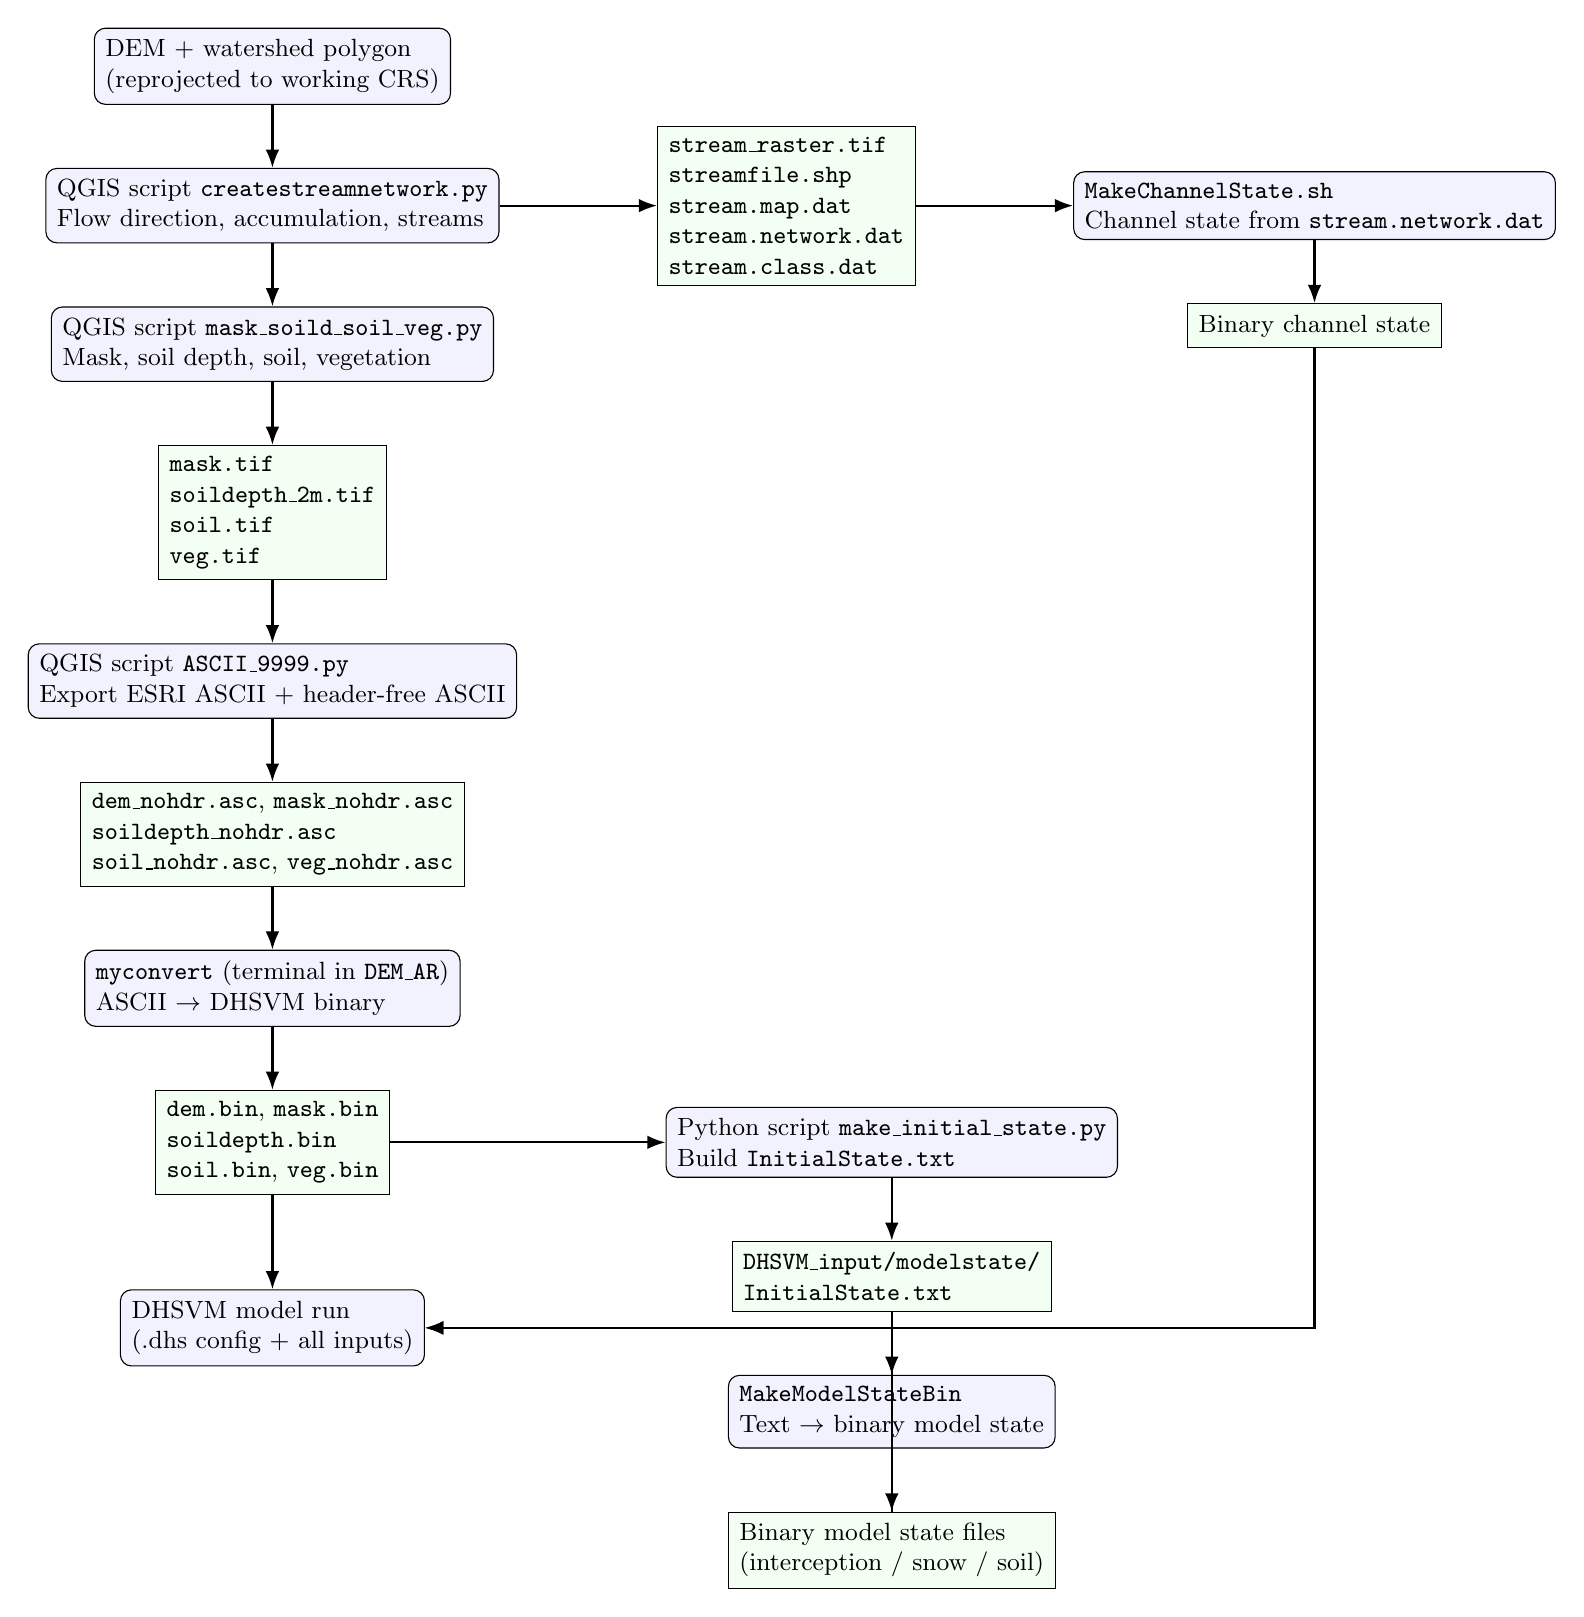
\begin{tikzpicture}[
  node distance=8mm and 15mm,
  >=Latex,
  process/.style={rectangle, rounded corners, draw, align=left, fill=blue!5, font=\small, inner sep=4pt},
  data/.style={rectangle, draw, align=left, fill=green!5, font=\small, inner sep=4pt},
  arrow/.style={->, thick}
]
\node[process] (start) {DEM + watershed polygon\\(reprojected to working CRS)};
\node[process, below=of start] (qgis1) {QGIS script \texttt{createstreamnetwork.py}\\Flow direction, accumulation, streams};
\node[data, right=20mm of qgis1] (streamfiles) {\texttt{stream\_raster.tif}\\\texttt{streamfile.shp}\\\texttt{stream.map.dat}\\\texttt{stream.network.dat}\\\texttt{stream.class.dat}};
\node[process, below=of qgis1] (qgis2) {QGIS script \texttt{mask\_soild\_soil\_veg.py}\\Mask, soil depth, soil, vegetation};
\node[data, below=of qgis2] (tifs) {\texttt{mask.tif}\\\texttt{soildepth\_2m.tif}\\\texttt{soil.tif}\\\texttt{veg.tif}};
\node[process, below=of tifs] (ascii) {QGIS script \texttt{ASCII\_9999.py}\\Export ESRI ASCII + header-free ASCII};
\node[data, below=of ascii] (ascfiles) {\texttt{dem\_nohdr.asc}, \texttt{mask\_nohdr.asc}\\\texttt{soildepth\_nohdr.asc}\\\texttt{soil\_nohdr.asc}, \texttt{veg\_nohdr.asc}};
\node[process, below=of ascfiles] (myconvert) {\texttt{myconvert} (terminal in \texttt{DEM\_AR})\\ASCII $\rightarrow$ DHSVM binary};
\node[data, below=of myconvert] (bins) {\texttt{dem.bin}, \texttt{mask.bin}\\\texttt{soildepth.bin}\\\texttt{soil.bin}, \texttt{veg.bin}};
\node[process, right=35mm of bins] (initpy) {Python script \texttt{make\_initial\_state.py}\\Build \texttt{InitialState.txt}};
\node[data, below=of initpy] (inittext) {\texttt{DHSVM\_input/modelstate/}\\\texttt{InitialState.txt}};
\node[process, below=of inittext] (mkstate) {\texttt{MakeModelStateBin}\\Text $\rightarrow$ binary model state};
\node[data, below=of mkstate] (statebin) {Binary model state files\\(interception / snow / soil)};
\node[process, right=20mm of streamfiles] (mkch) {\texttt{MakeChannelState.sh}\\Channel state from \texttt{stream.network.dat}};
\node[data, below=of mkch] (chbin) {Binary channel state};
\node[process, below=12mm of bins] (dhs) {DHSVM model run\\(.dhs config + all inputs)};
\draw[arrow] (start) -- (qgis1);
\draw[arrow] (qgis1) -- (streamfiles);
\draw[arrow] (qgis1) -- (qgis2);
\draw[arrow] (qgis2) -- (tifs);
\draw[arrow] (tifs) -- (ascii);
\draw[arrow] (ascii) -- (ascfiles);
\draw[arrow] (ascfiles) -- (myconvert);
\draw[arrow] (myconvert) -- (bins);
\draw[arrow] (bins) -- (dhs);
\draw[arrow] (streamfiles) -- (mkch);
\draw[arrow] (mkch) -- (chbin);
\draw[arrow] (chbin) |- (dhs);
\draw[arrow] (bins.east) -- ++(8mm,0) |- (initpy.west);
\draw[arrow] (initpy) -- (inittext);
\draw[arrow] (inittext) -- (mkstate);
\draw[arrow] (mkstate) -- (statebin);
\draw[arrow] (statebin) |- (dhs);
\end{tikzpicture}
\end{document}
